\section{Results and Discussion}

This section presents the performance of the developed models for patient deterioration classification and specialized Natural Language Processing (NLP) tasks. AI-generated interpretations are integrated throughout to provide deeper insights into the results.

\subsection{Patient Deterioration Classification Results}

The primary objective of this sub-task was to accurately classify patient deterioration. A range of models were developed and rigorously evaluated using standard metrics, including Accuracy, Precision, Recall, F1-score, and Area Under the Receiver Operating Characteristic Curve (AUC), to determine their predictive capabilities.

\subsubsection{Performance of Traditional Models (\textit{Random Forest, XGBoost, Neural Networks}) and Transformer-based Tabular Models (\textit{TabTransformer, FT Transformer})}

The performance metrics for several traditional machine learning models (\textit{Random Forest, XGBoost, Neural Network}) and transformer-based models adapted for tabular data (\textit{FT Transformer \parencite{gorishniy2023revisitingdeeplearningmodels}, Tab Transformer \parencite{huang2020tabtransformertabulardatamodeling}}) were evaluated on the designated test set. The evaluated matrices are displayed in the Table \ref{tab:ml_model_performance}  below.

\begin{table}[htbp]
    \centering
    \caption{Performance Metrics of Machine Learning Models}
    \label{tab:ml_model_performance}
    \begin{tabular}{lccccc}
        \hline
        \textbf{Model} & \textbf{Accuracy} & \textbf{Precision} & \textbf{Recall} & \textbf{F1} & \textbf{AUC} \\
        \hline
        Random Forest & 0.994 & 0.994 & 0.994 & 0.994 & 1.000 \\
        XGBoost & 0.989 & 0.988 & 0.988 & 0.988 & 0.999 \\
        Neural Network & 0.992 & 0.988 & 0.994 & 0.991 & 0.999 \\
        FT Transformer & 0.992 & 0.988 & 0.994 & 0.991 & 1.000 \\
        Tab Transformer & 0.986 & 0.977 & 0.994 & 0.986 & 1.000 \\
        \hline
    \end{tabular}
\end{table}

Further visualization of model performance was achieved through confusion matrices, Figure \ref{fig:confusion_matrices_ml} and AUC curve, Figure \ref{fig:roc_curves_ml}. These visualizations provide a more granular view of each model's classification behavior and discrimination ability.

\begin{figure}[httpb] % 'b' places the figure at the bottom of the page
    \centering
    \begin{minipage}{0.45\textwidth}
        \centering
        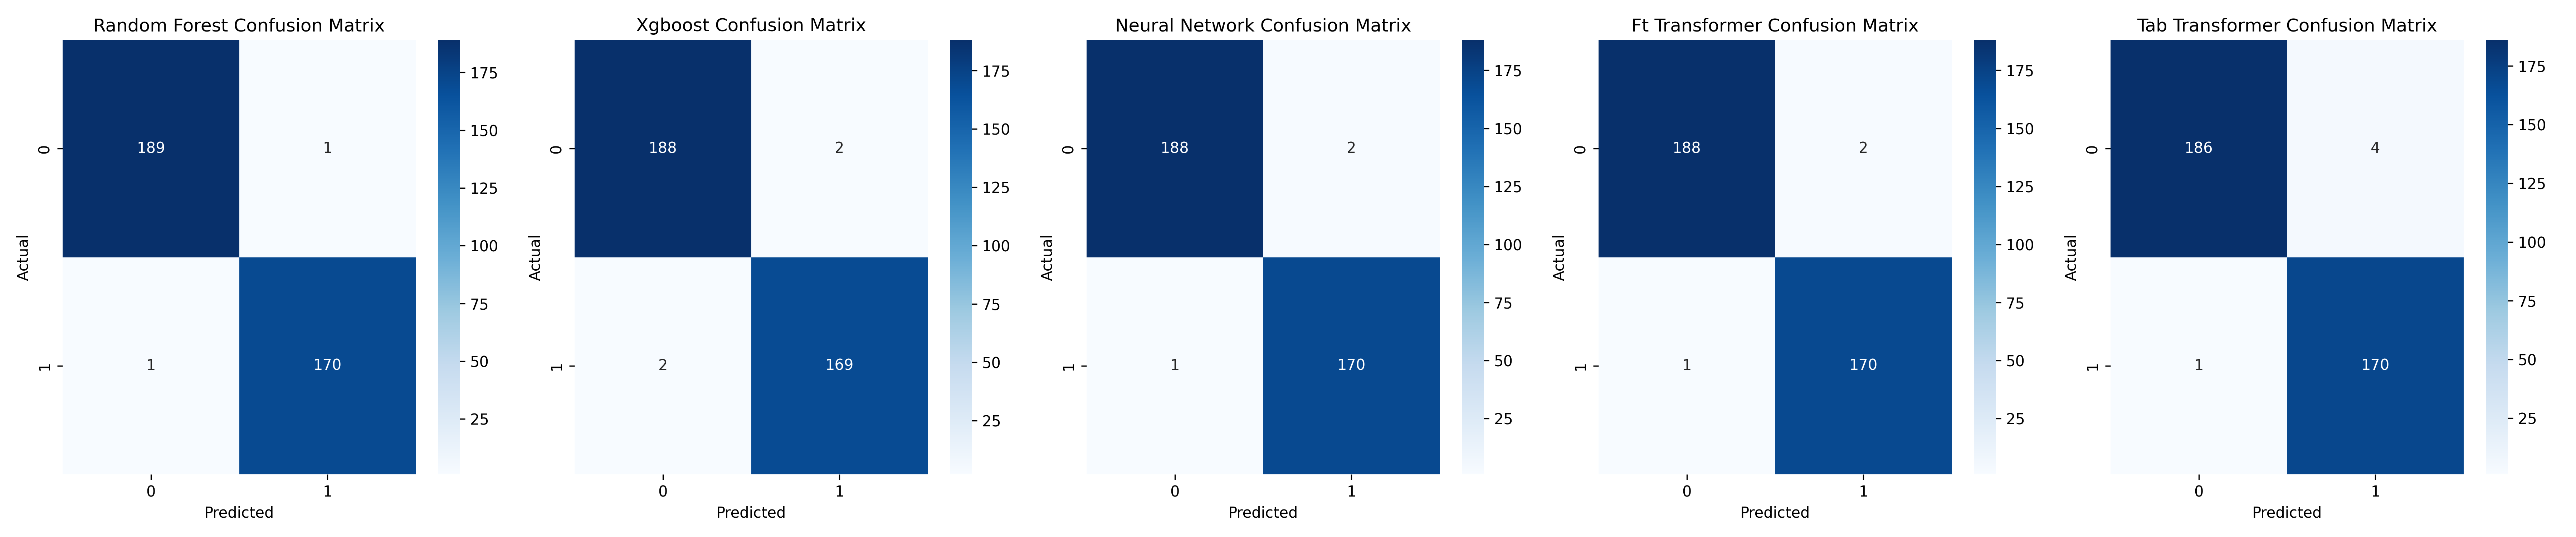
\includegraphics[width=\textwidth]{../images/ml_confusion_matrices.png} % Replace with your first image path
        \caption{Confusion Matrices}
        \label{fig:confusion_matrices_ml}
    \end{minipage}
    \hfill
    \begin{minipage}{0.45\textwidth}
        \centering
        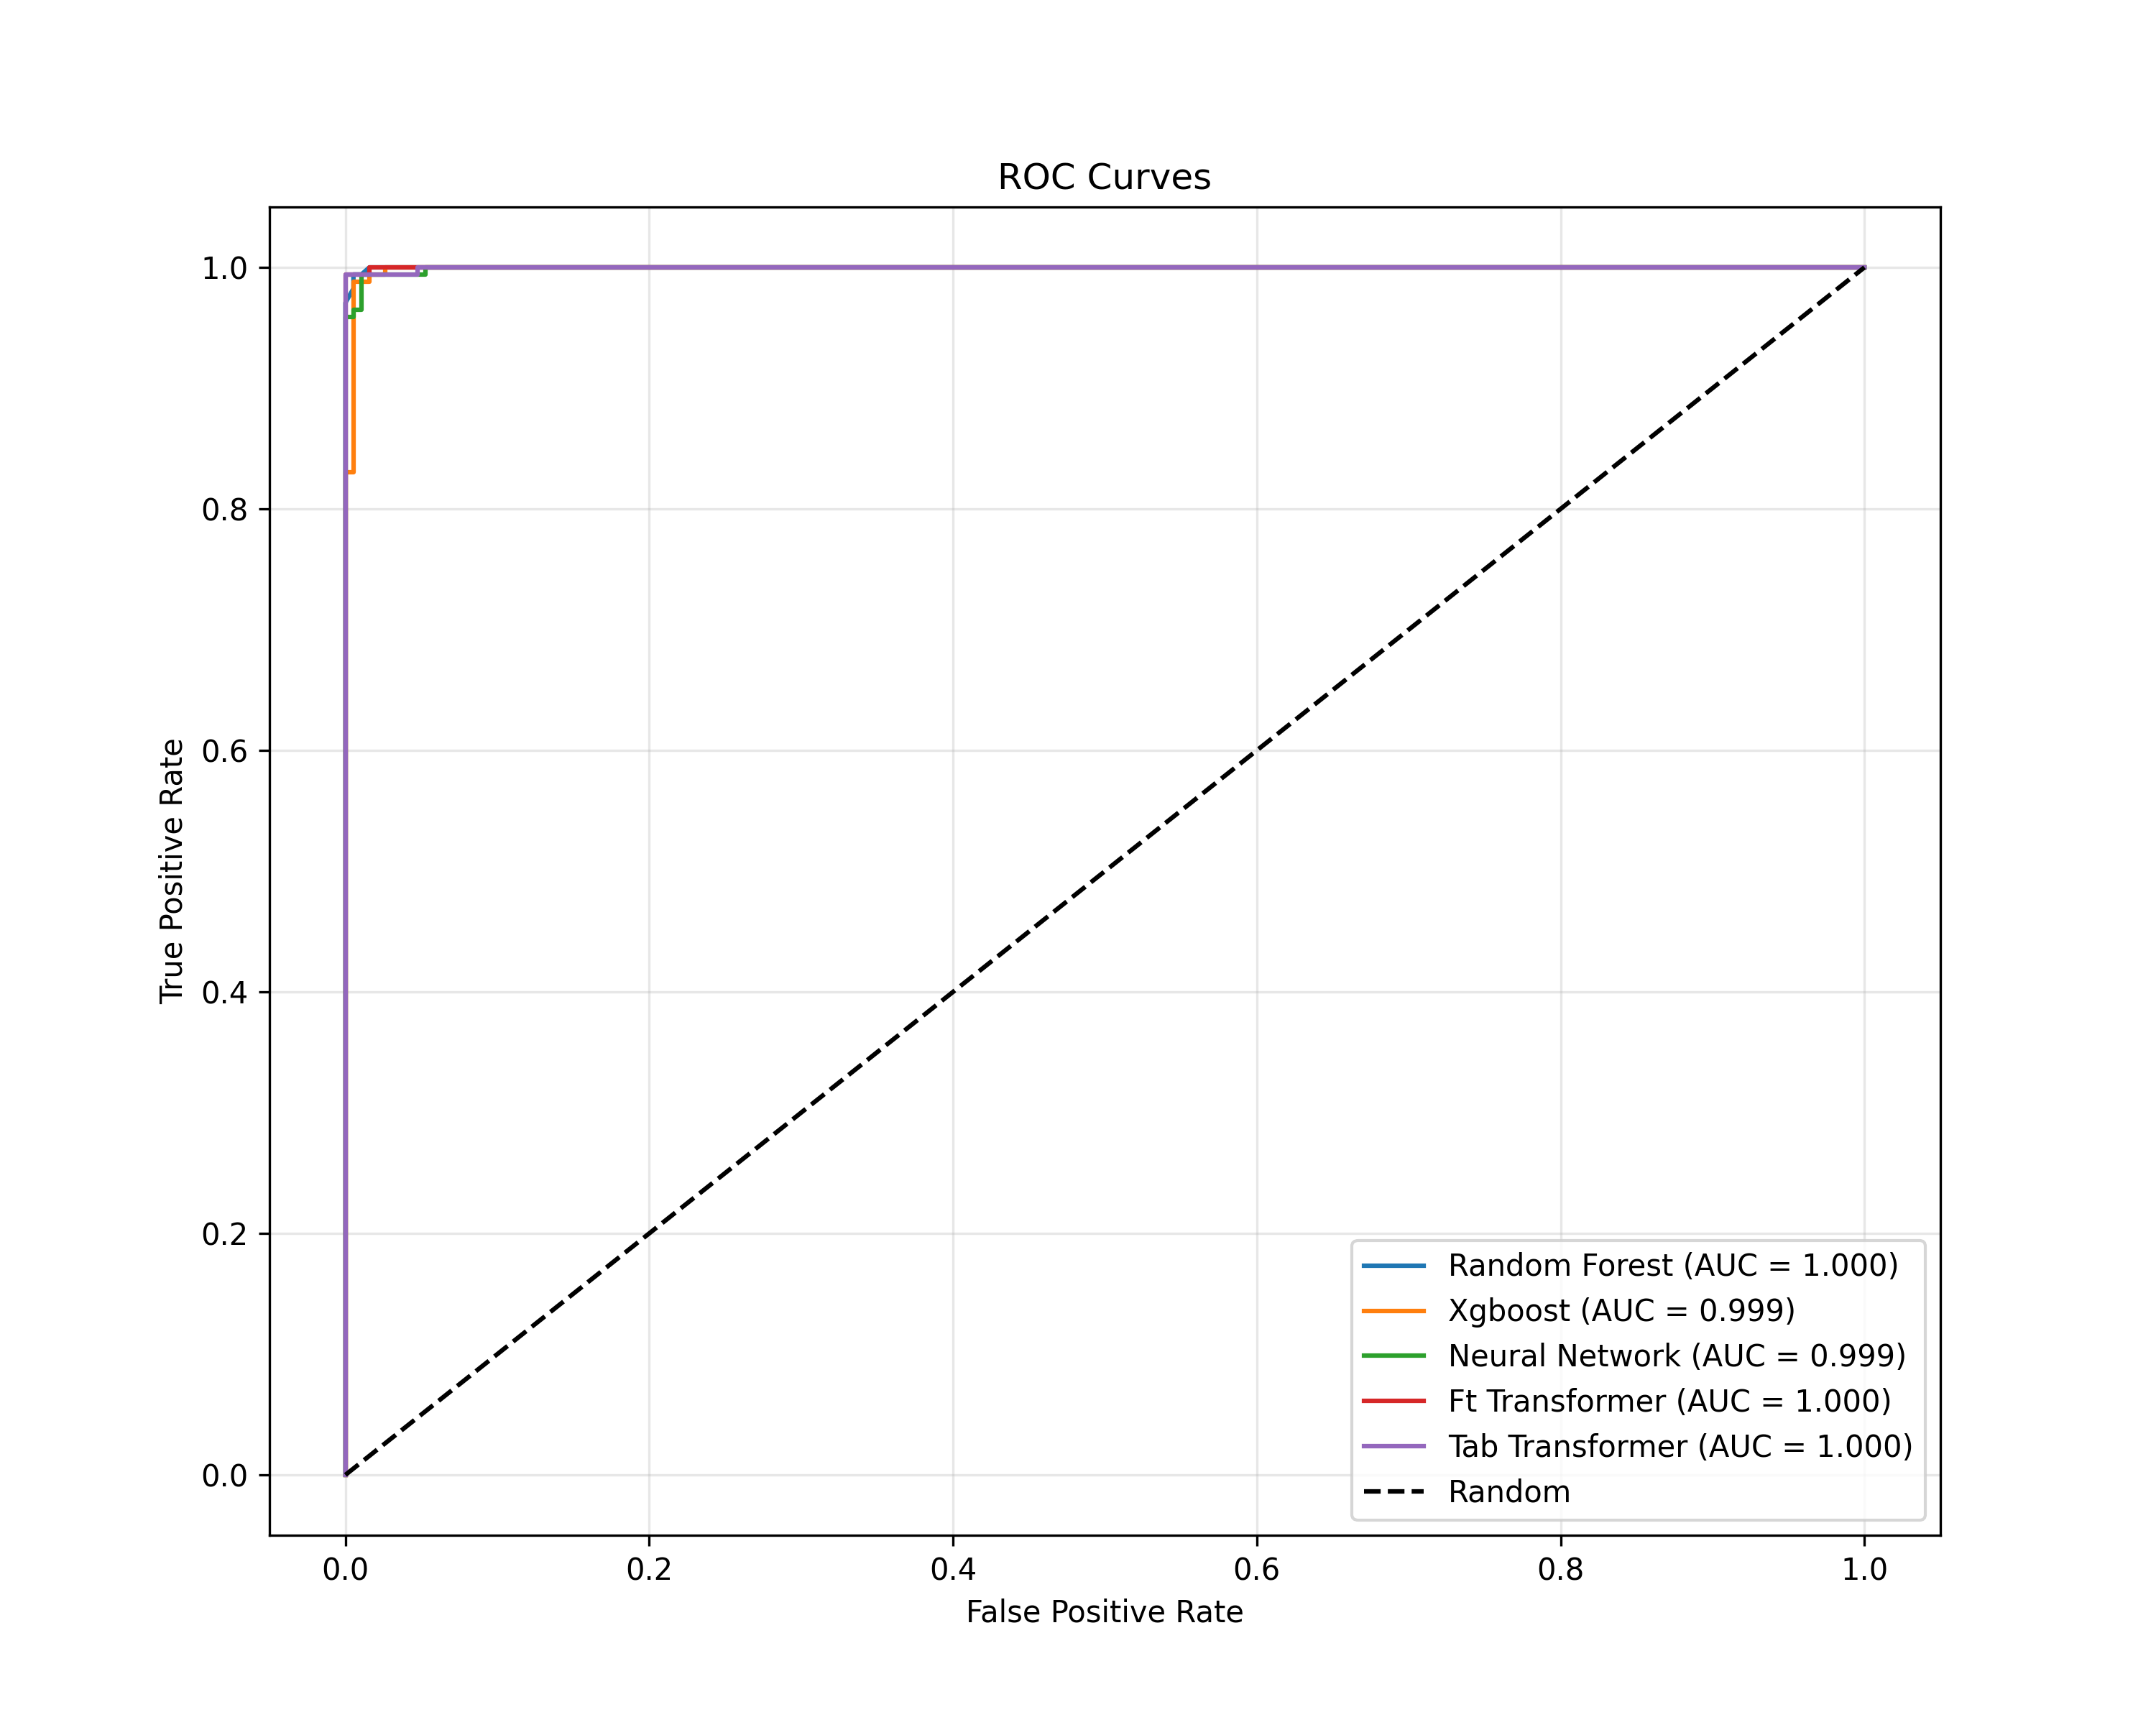
\includegraphics[width=\textwidth]{../images/ml_roc_curves.png} % Replace with your second image path
        \caption{ROC Curves}
        \label{fig:roc_curves_ml}
    \end{minipage}
\end{figure}

\subsubsection{AI-Assisted Interpretation of Deterioration Classification Results}

To augment the analysis, an AI model (\textit{Gemini-2.5-Flash-Thinking-Preview-0417}) \parencite{Doshi_2025} was employed to interpret the performance metrics table. We identified Random Forest as the best overall performer, attributing this to its superior accuracy, precision, recall, and F1-score, alongside a highly competitive AUC. While FT Transformer exhibited a marginally higher AUC, we noticed Random Forest's balanced and consistently high scores across various threshold-dependent metrics. Comparing traditional and deep learning approaches, we noted that traditional tree-based models, particularly Random Forest and XGBoost, were highly competitive, with Random Forest leading. Among the deep learning models, FT Transformer achieved the best AUC, whereas Tab Transformer registered the lowest accuracy, precision, and F1-score. We attributed these performance differences to factors such as model suitability for tabular data (where tree-based models often excel), the capacity to capture complex feature interactions, model robustness (often enhanced by ensemble methods), the effectiveness of hyperparameter tuning, and the influence of data size. For further improvement, we suggested avenues including more rigorous hyperparameter tuning, comprehensive cross-validation, advanced feature engineering, the exploration of ensembling or stacking techniques, and fine-tuning of classification thresholds. Based on its analysis, the AI recommended Random Forest for potential deployment, citing its leading performance, inherent robustness, computational efficiency, and comparatively better interpretability in this context relative to the deep learning alternatives.

The AI's interpretation of the confusion matrices, based on raw True Negative (TN), False Positive (FP), False Negative (FN), and True Positive (TP) values, involved a recalculation of accuracy, precision, recall, and F1-scores. This re-evaluation positioned both Random Forest and FT Transformer as top performers. Random Forest demonstrated excellence in precision and overall accuracy. Notably, FT Transformer achieved perfect recall, successfully identifying all positive cases while maintaining high accuracy and F1-score. Tab Transformer also showed perfect recall but at the cost of lower precision. In contrast, XGBoost generally performed the worst according to these raw confusion matrix-derived metrics. The AI concluded that the "best" model selection would depend on specific clinical priorities: FT Transformer would be favored if minimizing False Negatives is paramount, whereas Random Forest would be preferred for minimizing False Positives or achieving a balanced F1-score.

An AI-driven interpretation of the ROC curves revealed that Random Forest, FT Transformer, and Tab Transformer all achieved perfect AUC scores of 1.000. XGBoost and Neural Network also demonstrated exceptional performance with AUCs of 0.999. The AI highlighted that such high AUC values imply an excellent to perfect ability of the models to distinguish between positive and negative classes on the evaluated dataset. However, these near-perfect scores prompted caution from the AI, which raised concerns regarding potential data leakage, overfitting (particularly if evaluation sets were small or cross-validation was not rigorously applied), or the possibility of a trivially easy dataset. Given that perfect scores were observed across multiple diverse architectures, data leakage was identified as a strong possibility requiring thorough investigation. The AI's report concluded that while all models exhibited outstanding performance on the provided evaluation set, the perfect or near-perfect AUCs warrant careful examination of potential underlying data issues before definitive conclusions about model robustness and generalizability can be drawn.

\subsubsection{Comparative Analysis and Discussion}

The models developed for patient deterioration classification generally demonstrated exceptionally high performance. As highlighted by both the initial results table and the AI's interpretation, the Random Forest model exhibited the most consistent and superior performance across accuracy, precision, recall, and F1-score. The FT Transformer also emerged as a strong contender, particularly distinguished by its leading AUC value.

The AI's recalculation of metrics directly from raw confusion matrix values offered a slightly more nuanced perspective, elevating FT Transformer to a similar top-tier status as Random Forest, with specific commendation for FT Transformer's perfect recall. This underscores that the interpretation of "best" performance can subtly shift depending on whether raw confusion matrix counts, pre-calculated metrics, or specific evaluation priorities (e.g., threshold-independent AUC versus threshold-dependent F1-score) are emphasized.

The achievement of perfect AUCs by three models—Random Forest, FT Transformer, and Tab Transformer—is particularly striking. As the AI interpretation correctly pointed out, such perfect scores, especially in a biomedical context even with simulated data, necessitate a meticulous review of the data generation, feature engineering, and data splitting processes. This review is crucial to rule out any form of data leakage or the creation of an overly simplistic classification task that might not accurately reflect real-world complexities. If these high scores are indeed genuine and the task is inherently highly separable with the given features, it would indicate that these models are exceptionally effective. Nevertheless, caution is advised. Further validation on more challenging, diverse, or independently generated datasets would be highly beneficial to confirm these findings. It is plausible that the engineered features derived from questionnaires and medical history significantly contributed to this high degree of separability observed in the data.

\subsection{NLP Task Results}

This section details the performance of models developed for various NLP tasks, including sentiment analysis, clinical text interpretation (Named Entity Recognition), and questionnaire response classification, again incorporating AI-assisted interpretations.

\subsubsection{Sentiment Analysis on \texttt{describe\_lifestyle}}

For sentiment analysis, models were applied to the \texttt{describe\_lifestyle} text from questionnaire responses. Evaluation results which encompassed metrics for Fatigue, Activity/Anxiety, and Mental Health sentiment. The underlying models were BERT base, fine-tuned for 3-class sentiment classification (positive, neutral, negative). Visualizations included confusion matrices and ROC curves as well as training loss curves. The summary of evaluation metrics is presented in Table \ref{tab:sentiment_analysis_performance} below:

\begin{table}[htbp]
    \centering
    \caption{Performance Metrics of Sentiment Analysis Models}
    \label{tab:sentiment_analysis_performance}
    \begin{tabular}{lccccc}
        \hline
        \textbf{Model} & \textbf{Accuracy} & \textbf{Precision} & \textbf{Recall} & \textbf{F1-Score} & \textbf{AUC} \\
        \hline
        Fatigue & 0.917 & 0.922 & 0.917 & 0.918 & 0.923 \\
        Activity & 0.884 & 0.881 & 0.884 & 0.882 & 0.887 \\
        Mental Health & 0.888 & 0.890 & 0.888 & 0.889 & 0.890 \\
        \hline
    \end{tabular}
\end{table}

AI-assisted interpretations provided further insights. The AI rated the AUC, Figure \ref{fig:confusion_matrices_sa} for Fatigue (0.92) as excellent, and those for Activity/Anxiety (0.89) and Mental Health (0.89) as very good, indicating strong discriminatory power for all models. Fatigue's superior performance was hypothesized to stem from potentially clearer linguistic patterns or less ambiguity within its associated dataset. Analysis of confusion matrices, Figure \ref{fig:roc_curves_sa} revealed that the Fatigue model performed excellently on True Positives and True Negatives, with its main weakness being the Neutral class. The Activity/Anxiety model was strong on True Negatives but struggled significantly with the Neutral class and exhibited more diffuse errors. The Mental Health model showed outstanding performance on True Positives, with its primary weakness also being the Neutral class. The AI also flagged "Activity" as a likely typo for "Anxiety." Class imbalance and sentiment overlap, especially concerning the "Neutral" category, were identified as potential contributing issues. Interpretation of the loss curves indicated that all models learned effectively from the training data. However, severe overfitting was observed early in training (around Epoch 2-3), Figure \ref{fig:loss_curves_sa} for all categories, evidenced by validation loss increasing or fluctuating while training loss continued to decrease. This suggested that training for the full 30 epochs was excessive, and early stopping at the best epoch (Epoch 2 or 3, depending on the category) was deemed crucial. The AI recommended strategies such as early stopping, regularization, acquiring more data, and adjusting learning rates to mitigate overfitting. The AI's interpretation of aggregated metrics confirmed the Fatigue model as the strongest performer across all metrics, with Mental Health slightly outperforming Activity. While these aggregate metrics aligned with ROC and confusion matrix findings, they tended to mask per-class struggles, particularly with the 'Moderate Risk' (likely corresponding to 'Neutral' sentiment) class. Limitations due to the small dataset size and the inherent subjectivity of questionnaire data were also noted by the AI.

\begin{figure}[httpb] % 'b' places the figure at the bottom of the page
    \centering
    \begin{minipage}{0.45\textwidth}
        \centering
        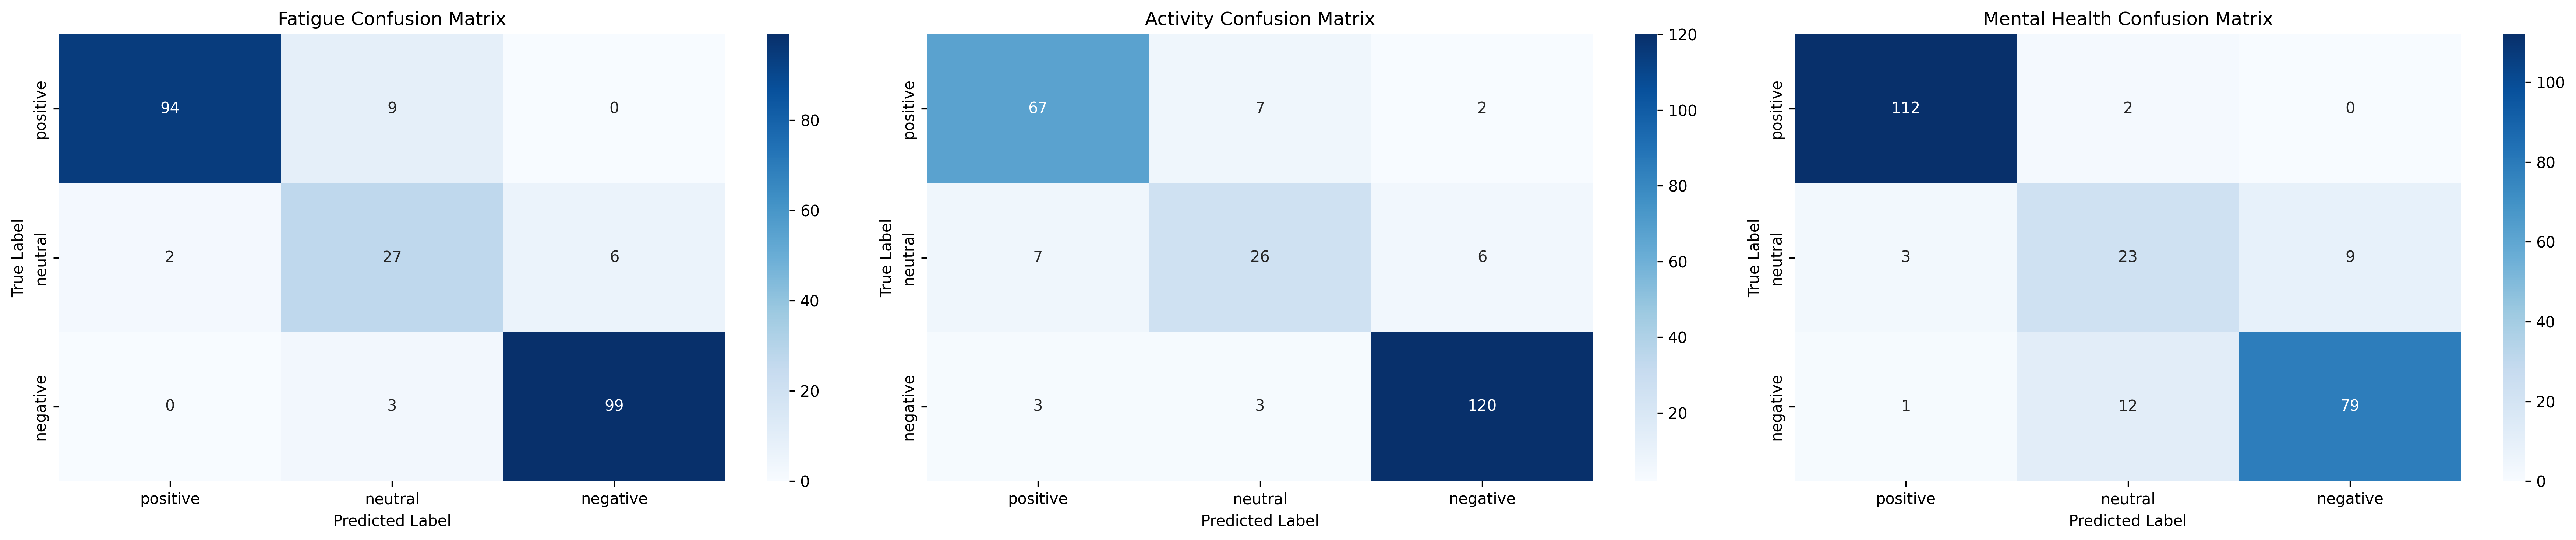
\includegraphics[width=\textwidth]{../images/sa_confusion_matrices.png} % Replace with your first image path
        \caption{Confusion Matrices}
        \label{fig:confusion_matrices_sa}
    \end{minipage}
    \hfill
    \begin{minipage}{0.45\textwidth}
        \centering
        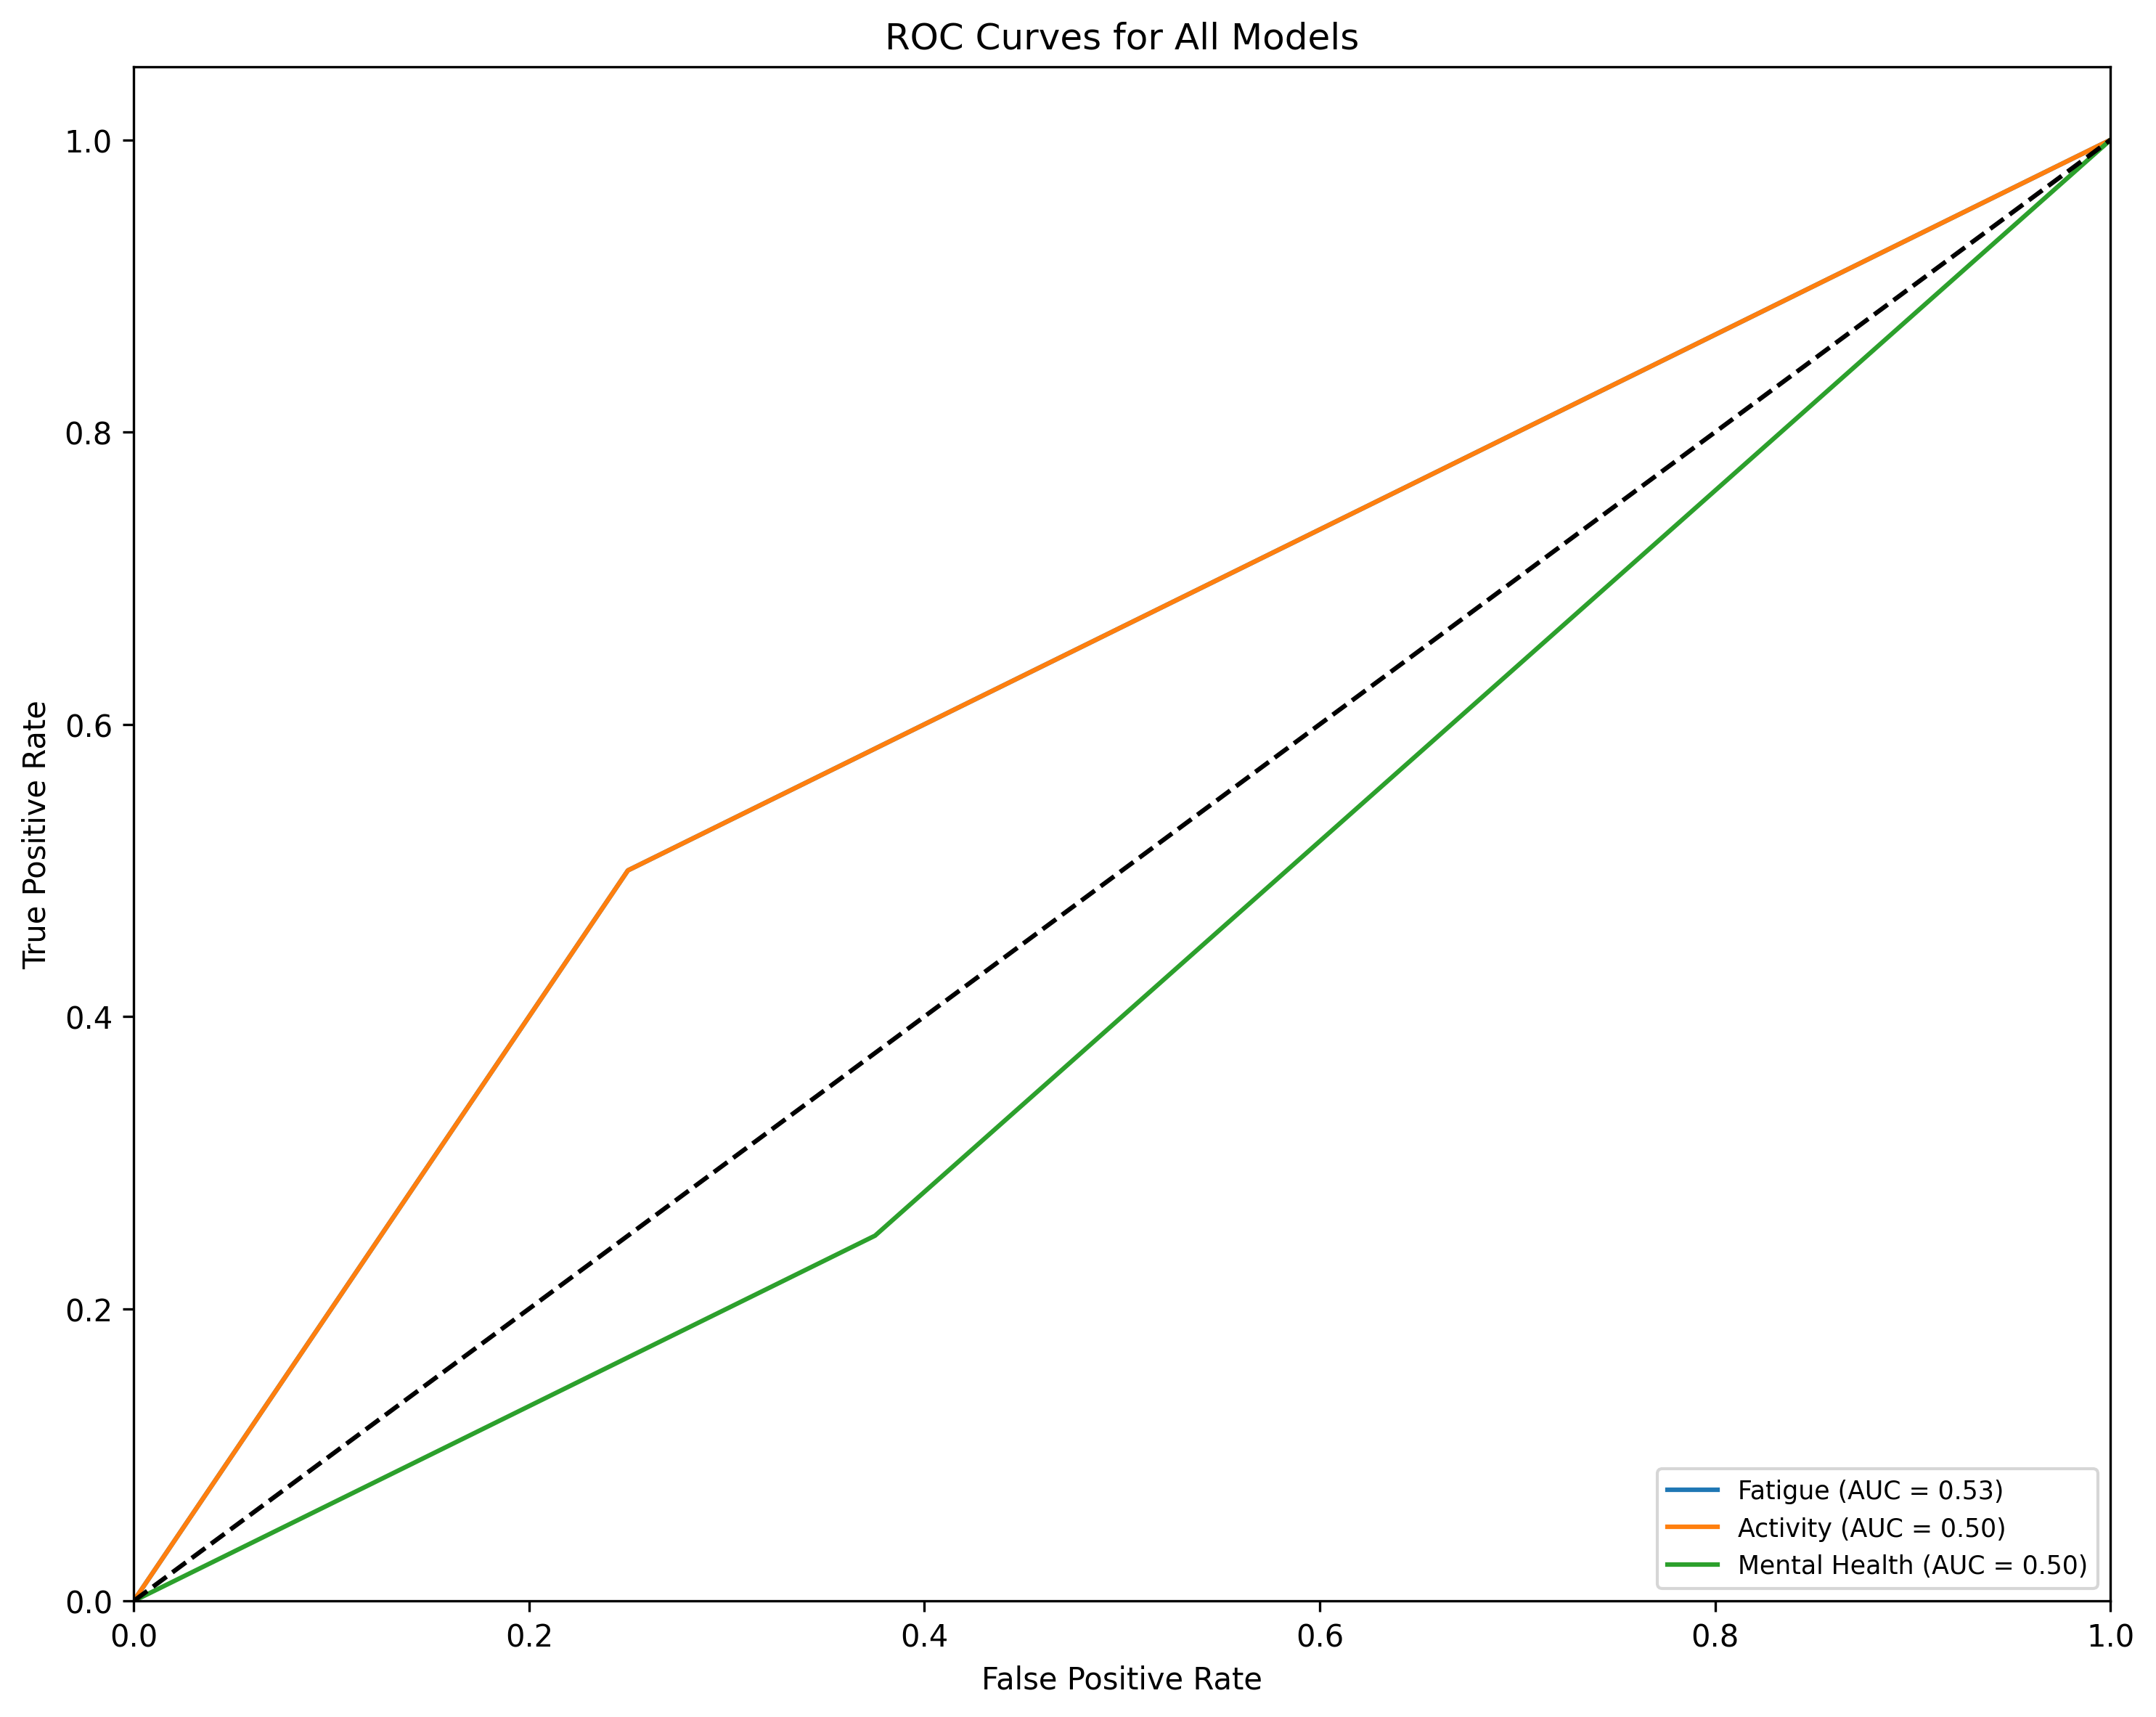
\includegraphics[width=\textwidth]{../images/sa_roc_curves.png} % Replace with your second image path
        \caption{ROC Curves}
        \label{fig:roc_curves_sa}
    \end{minipage}
\end{figure}

\begin{figure}[htpb]
    \centering
    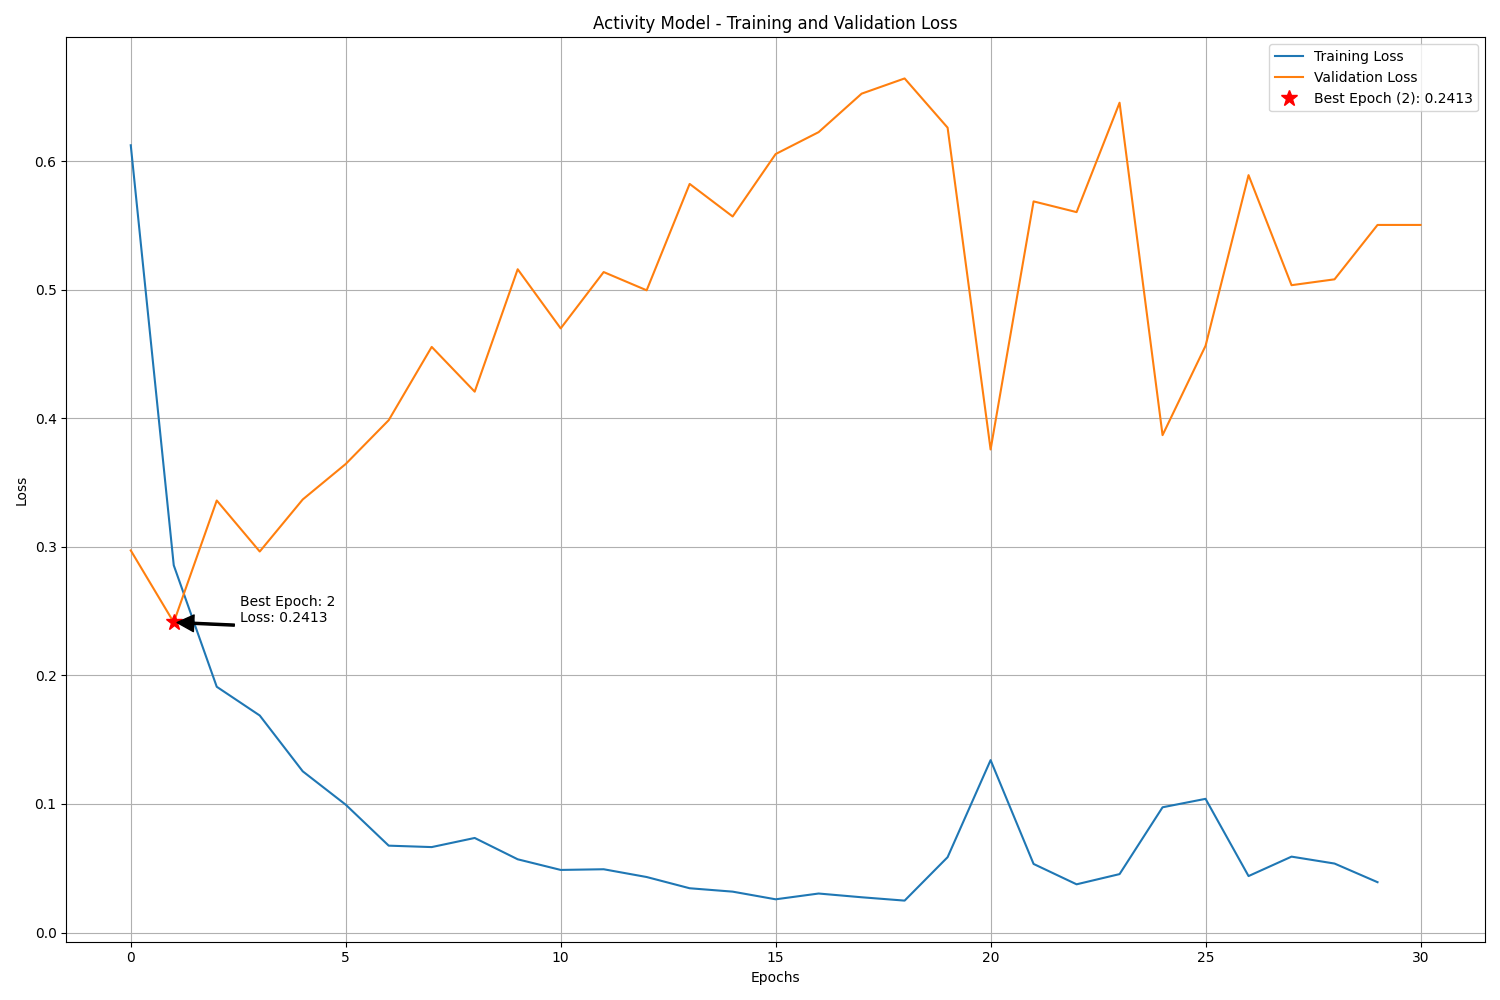
\includegraphics[width=0.4\textwidth]{../images/sa_loss_curves_with_best_epoch.png} % Replace with your image path
    \caption{Training Loss Curves with Best Epoch}
    \label{fig:loss_curves_sa}
\end{figure}

In discussion, the BERT base models demonstrated commendable performance in sentiment analysis, particularly for the Fatigue category. A consistent challenge across all sentiment categories was the classification of "Neutral" sentiment, a common difficulty in NLP tasks due to its subjective nature and often subtle linguistic expression. The early and pronounced overfitting highlighted by the AI's analysis of loss curves suggests that even robust models like BERT base can quickly memorize training examples when datasets are small, underscoring the critical importance of careful early stopping procedures.

\subsubsection{Clinical Text Interpretation (NER) on medical\_history}

Named Entity Recognition (NER) was performed on medical\_history text using a fine-tuned Bio-Clinical BERT model. The notebook loaded NER evaluation results in cell 497826f3, summarized in the Metrics Table \ref{tab:ner_performance} below:

\begin{table}[htbp]
    \centering
    \caption{Performance Metrics of Named Entity Recognition Model}
    \label{tab:ner_performance}
    \begin{tabular}{lccccc}
        \hline
        \textbf{Model} & \textbf{Accuracy} & \textbf{Precision} & \textbf{Recall} & \textbf{F1-Score} & \textbf{AUC} \\
        \hline
        Bio-Clinical BERT & 0.998 & 0.908 & 0.943 & 0.926 & 1.000 \\
        \hline
    \end{tabular}
\end{table}

The ROC curve, Figure \ref{fig:ner_roc_curve} for this task indicated an AUC of 1.00. Training curves, Figure \ref{fig:ner_training_curves}, provided insights into the learning process.

\begin{figure}[httpb] % 'b' places the figure at the bottom of the page
    \centering
    \begin{minipage}{0.45\textwidth}
        \centering
        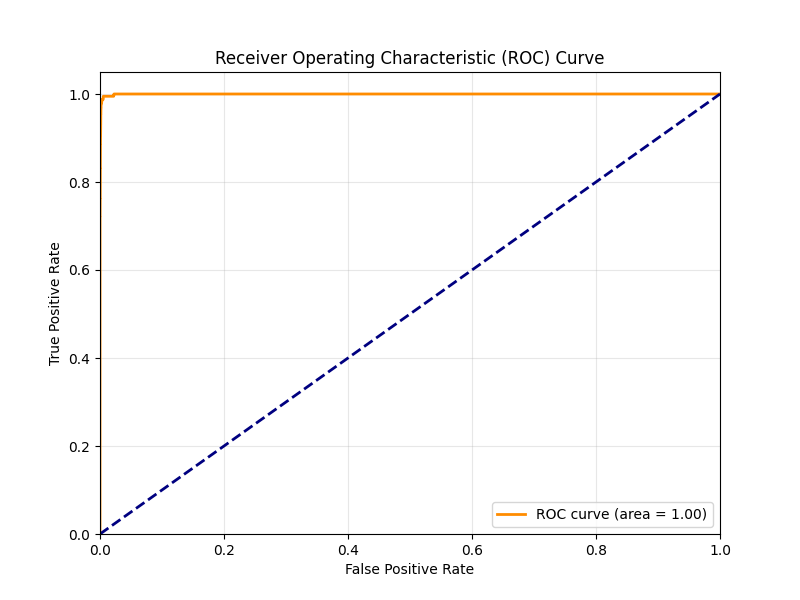
\includegraphics[width=\textwidth]{../images/ner_roc_curve.png} % Replace with your first image path
        \caption{ROC Curve}
        \label{fig:ner_roc_curve}
    \end{minipage}
    \hfill
    \begin{minipage}{0.45\textwidth}
        \centering
        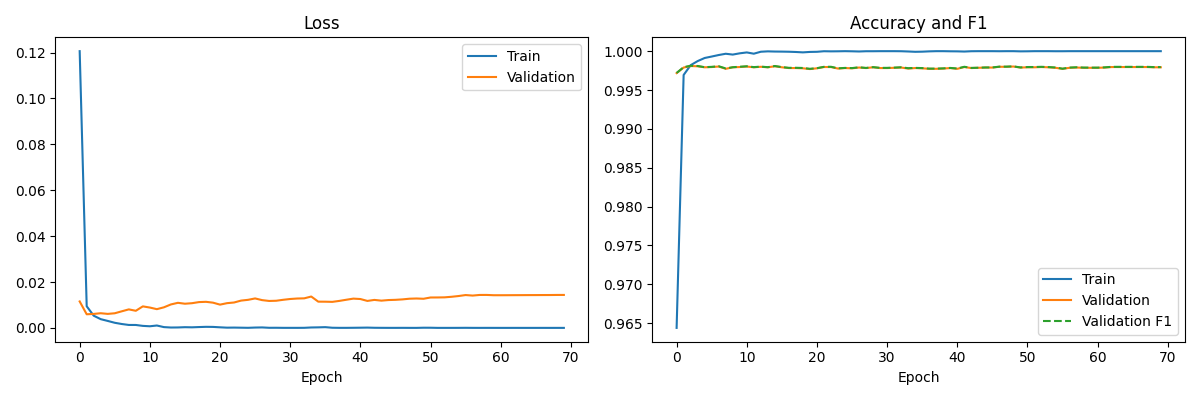
\includegraphics[width=\textwidth]{../images/ner_training_curves.png} % Replace with your second image path
        \caption{Training Curves}
        \label{fig:ner_training_curves}
    \end{minipage}
\end{figure}

AI-assisted interpretations offered a detailed analysis. The AI noted the exceptionally high accuracy (99.8\%), high F1-score (92.6\%), excellent recall (94.3\%), and good precision (90.8\%). The AUC (0.9996 from the Table \ref{tab:ner_performance}, 1.00 from the Figure \ref{fig:ner_roc_curve}) suggested near-perfect discriminative power at the token level for identifying entity tokens versus non-entity tokens. The AI cautioned that the high accuracy could be influenced by the preponderance of non-entity tokens (the "O" tag in IOB notation). High recall was deemed crucial for minimizing missed entities, while high precision indicated that most extracted entities were correct, with a slight observed preference for recall over precision. The AI's interpretation of the ROC curve, showing an AUC of 1.00 (or 0.9996), pointed to a perfect or near-perfect classifier at the token level. However, this perfect score again raised concerns about potential data leakage or an overly simplistic sub-problem, especially considering the high performance across other metrics. The AI's analysis of the training curves revealed that training loss dropped rapidly to near zero, and training accuracy/F1 reached near 1.0 very quickly, indicating that the model had effectively mastered the training data. Validation loss also decreased but plateaued at a level higher than training loss, signaling some degree of overfitting. Validation accuracy and F1-score were extremely high (approximately 0.998). A significant discrepancy was highlighted by the AI between the validation F1-score (0.998) observed from these training plots and the test F1-score (0.926) reported from the independent test set. This disparity strongly suggested poor generalization from the (small) training/validation data to the test set, likely attributable to the very small dataset size (1000 data points for NER). Consequently, the AI's recommendations heavily emphasized the need for acquiring more data, employing data augmentation techniques, and implementing robust cross-validation, given the dataset limitations.

Discussing these findings, the Bio-Clinical BERT model demonstrated very high potential for NER on disease entities. Token-level metrics such as Accuracy and the AUC derived from the ROC curve were near-perfect. However, the entity-level F1-score, while good at 0.926, was considerably lower than the F1-score observed on the validation set during training. This discrepancy highlights a common challenge when working with small datasets: a model can appear to perform almost perfectly on validation data but still struggle to generalize effectively to a truly independent test set, particularly for complex sequence labeling tasks like NER. The observed drop of approximately 7\% in F1-score indicates that while token-level classification might be excellent, consistently and correctly identifying the exact boundaries and types of entities on new, unseen data proves more challenging.

\subsubsection{Questionnaire Response Classification (\texttt{describe\_fatigue\_level, describe\_mental\_health})}

This task involved using BERT base models to classify textual questionnaire responses from \texttt{describe\_fatigue\_level} and \texttt{describe\_mental\_health} into "Low Risk," "Moderate Risk," and "High Risk" categories. The results and discussion for this appear to align closely with those presented for the "Sentiment Analysis" task, where "Fatigue," "Activity/Anxiety," and "Mental Health" were the evaluated categories with labels "positive," "neutral," and "negative." It is assumed that a mapping exists, such as "positive" to "Low Risk," "neutral" to "Moderate Risk," and "negative" to "High Risk," or a similar schema appropriate to the problem's framing. Therefore, the discussion from sentiment analysis largely applies here. Visual performance indicators for this specific framing are provided by confusion matrices, Figure \ref{fig:qr_confusion_matrices} and ROC curves, Figure \ref{fig:qr_roc_curves}.

\begin{figure}[httpb] % 'b' places the figure at the bottom of the page
    \centering
    \begin{minipage}{0.45\textwidth}
        \centering
        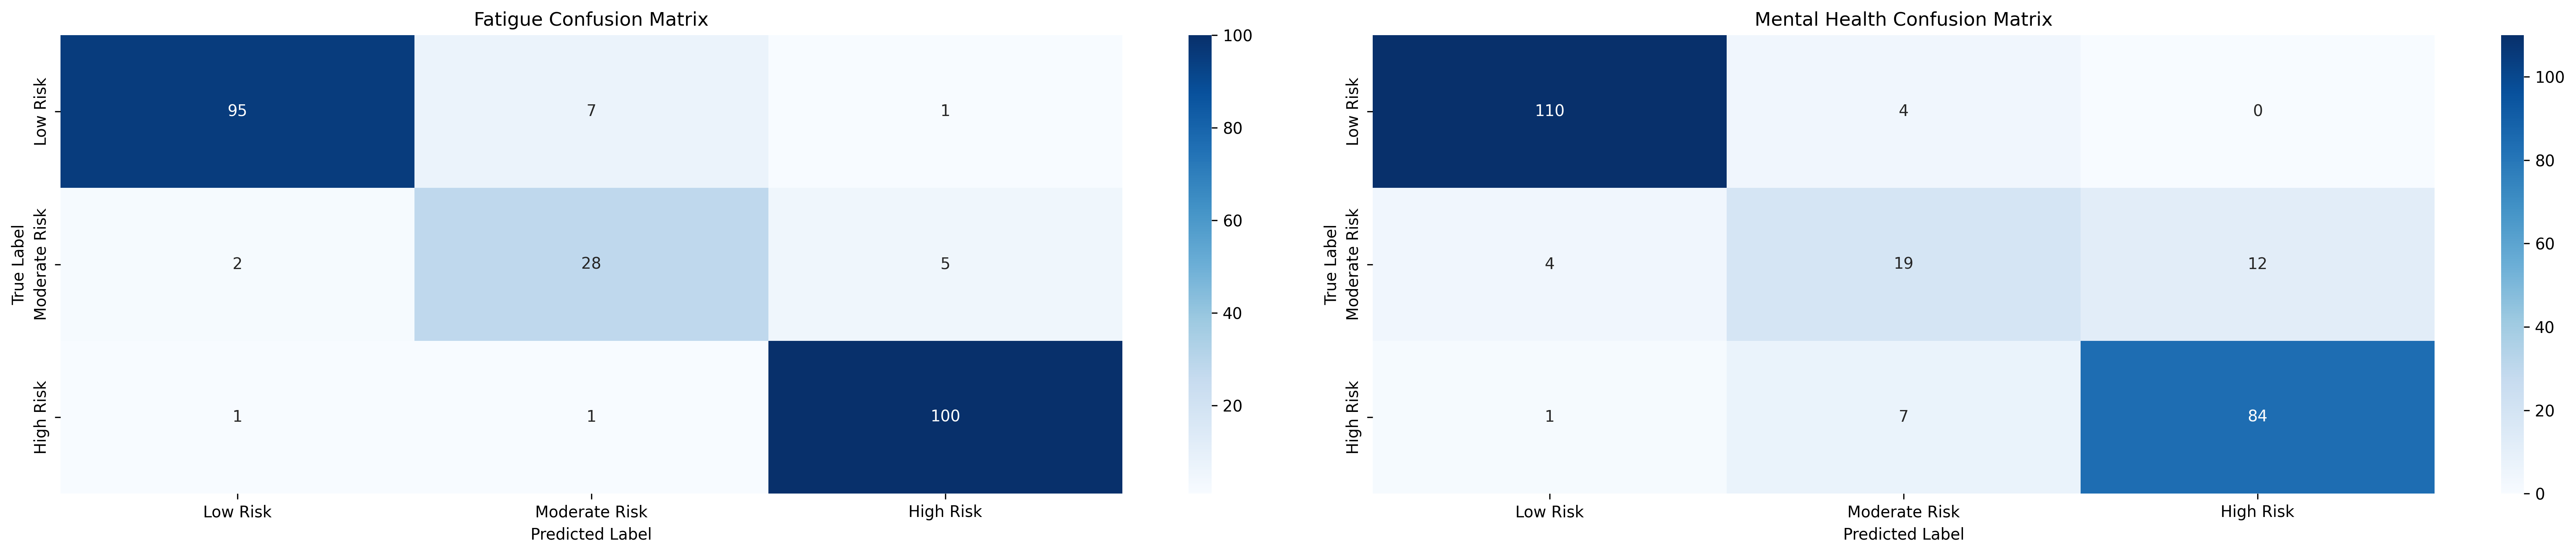
\includegraphics[width=\textwidth]{../images/qr_confusion_matrices.png} % Replace with your first image path
        \caption{Confusion Matrices}
        \label{fig:qr_confusion_matrices}
    \end{minipage}
    \hfill
    \begin{minipage}{0.45\textwidth}
        \centering
        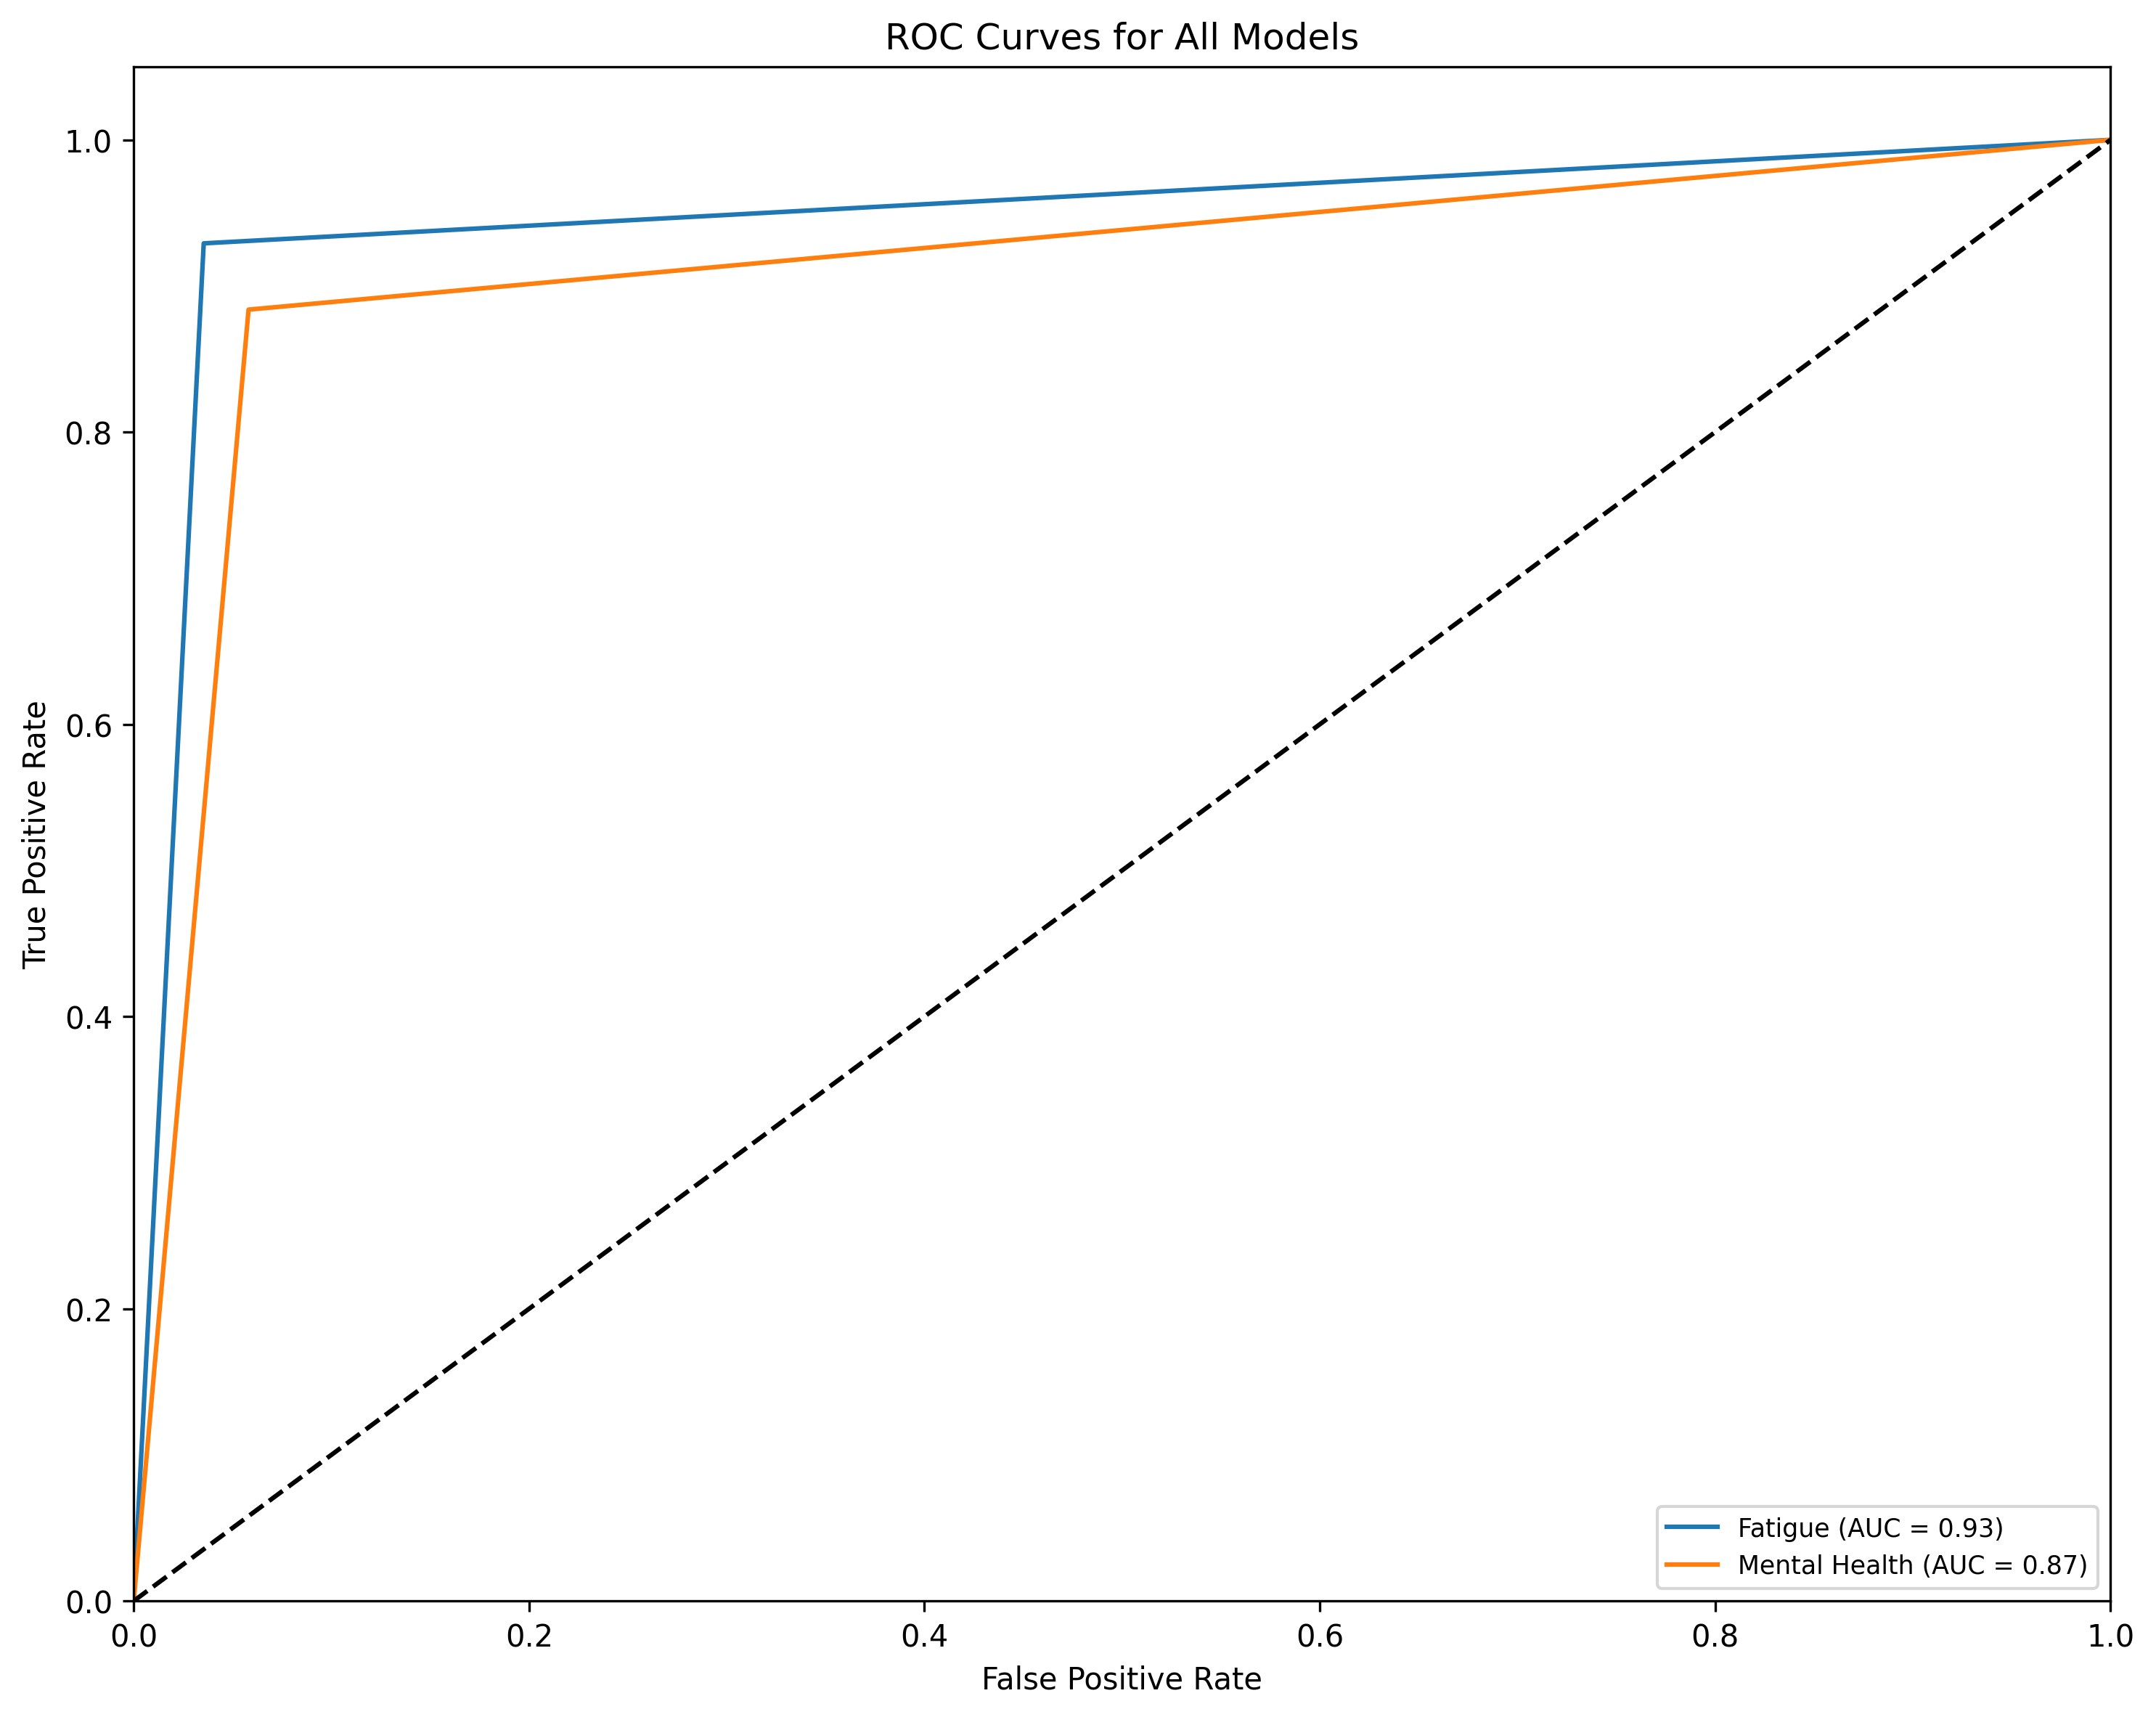
\includegraphics[width=\textwidth]{../images/qr_roc_curves.png} % Replace with your second image path
        \caption{ROC Curves}
        \label{fig:qr_roc_curves}
    \end{minipage}
\end{figure}

AI-assisted interpretation provided specific insights for this risk classification task. The AI calculated accuracies of approximately 92.9\% for Fatigue and 88.4\% for Mental Health from the confusion matrices. Both models demonstrated strength in identifying 'High Risk' cases (high recall). However, the 'Moderate Risk' class emerged as the weakest link for both models, suffering from numerous misclassifications into either 'Low' or 'High' risk categories. A critical error was noted for the Mental Health model, which misclassified 2 True High Risk cases as Low Risk. Class imbalance, with the 'Moderate Risk' category being smaller, was identified by the AI as a key contributing issue. Interpretation of the ROC curves indicated an AUC of 0.93 (excellent) for Fatigue and 0.87 (very good) for Mental Health, with the Fatigue model showing superior overall discriminative power. The AI also discussed limitations related to the small dataset size and the inherent nature of multi-class ROC calculation (e.g., reliance on One-vs-Rest averaging). The model evaluation metrics is shown in Table \ref{tab:questionnaire_risk_performance} below:

\begin{table}[htbp]
    \centering
    \caption{Performance Metrics of Questionnaire Risk Classification Models}
    \label{tab:questionnaire_risk_performance}
    \begin{tabular}{lccccc}
        \hline
        \textbf{Model} & \textbf{Accuracy} & \textbf{Precision} & \textbf{Recall} & \textbf{F1-Score} & \textbf{AUC} \\
        \hline
        Fatigue & 0.929 & 0.932 & 0.929 & 0.930 & 0.933 \\
        Mental Health & 0.884 & 0.877 & 0.884 & 0.878 & 0.871 \\
        \hline
    \end{tabular}
\end{table}

In summary, the BERT models were effective in stratifying risk levels based on textual questionnaire responses, particularly for the Fatigue category. The 'Moderate Risk' category consistently proved challenging, a common phenomenon in multi-class classification problems involving ordinal or subjective labels, often exacerbated by class imbalance. The observed performance disparity, Figure \ref{fig:qr_loss_curves} between the Fatigue and Mental Health models suggests that the linguistic cues indicative of fatigue risk might be more distinct or easier for the model to learn from the limited available data compared to those signaling mental health risk.

\begin{figure}[htpb]
    \centering
    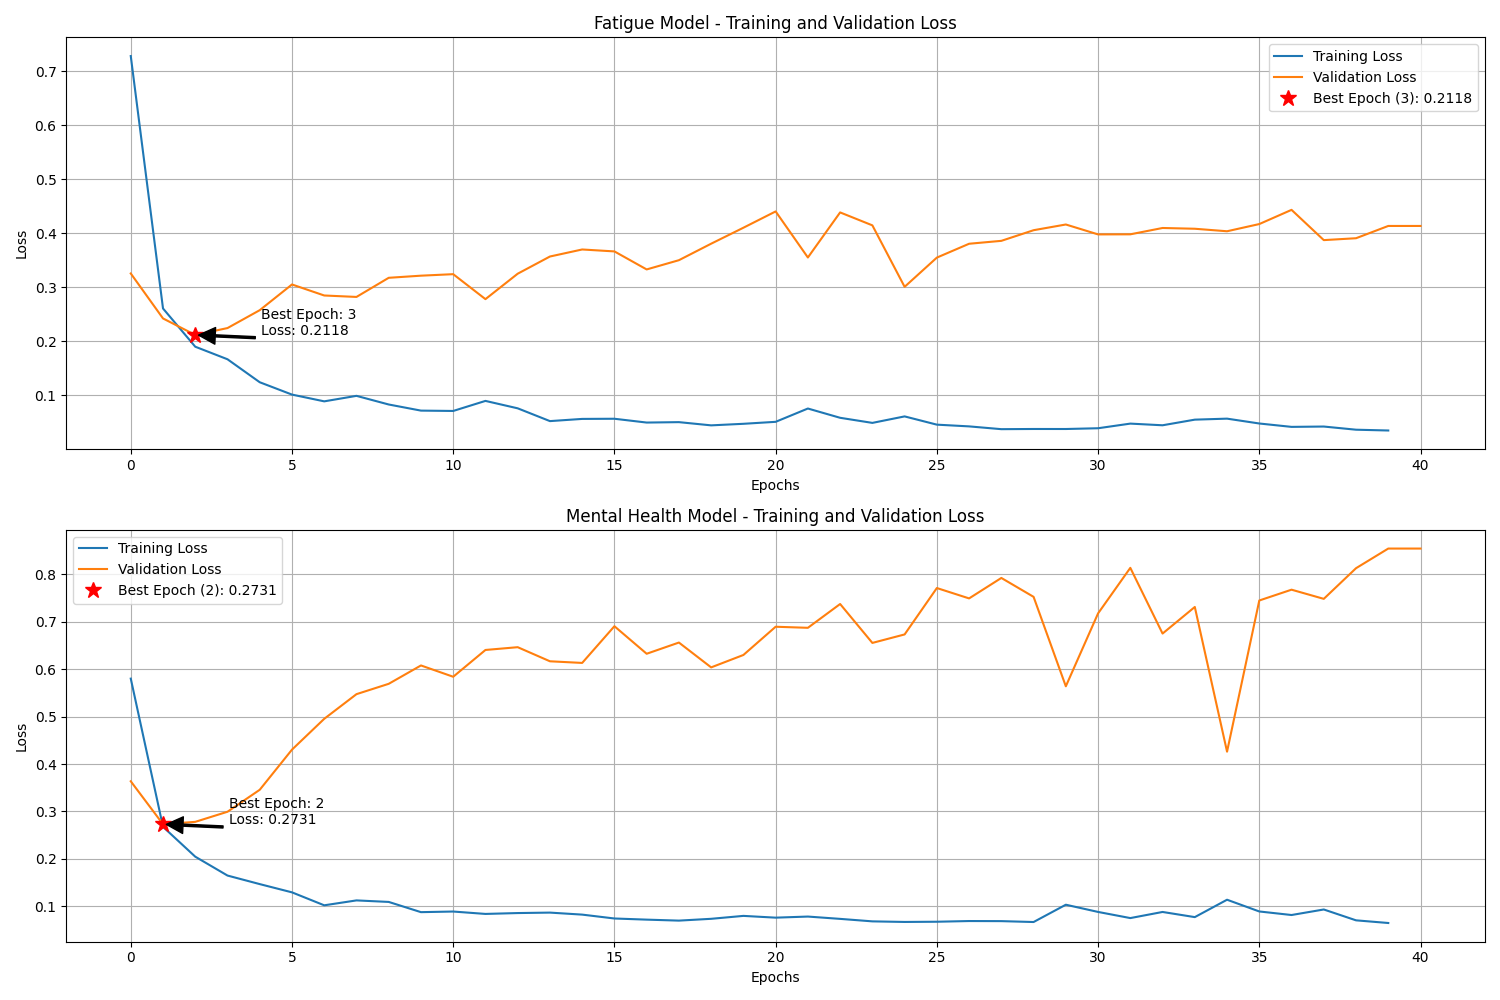
\includegraphics[width=0.4\textwidth]{../images/qr_loss_curves_with_best_epoch.png} % Replace with your image path
    \caption{Training Loss Curves with Best Epoch}
    \label{fig:qr_loss_curves}
\end{figure}

\subsection{Overall Discussion}

This section synthesizes the findings from both patient deterioration classification and the various NLP tasks, discussing their contributions, the role of generative AI and large language models, and persistent challenges.

The project successfully demonstrated the application of diverse AI models for the prediction of patient deterioration and a suite of related NLP tasks. Transformer-based models, notably FT Transformer for tabular data and various BERT variants for NLP applications, exhibited strong performance across their respective domains. The NLP tasks were crucial in generating quantifiable features, such as recognized disease entities from medical history (NER) and severity scores derived from questionnaire responses, as well as providing direct risk or sentiment classifications from free-text inputs.

While the contribution of NLP-derived features to the patient deterioration prediction models was not explicitly quantified through ablation studies in the provided notebook, their integral role is evident. Features engineered from \texttt{medical\_history} (e.g., extracted diseases via NER) and \texttt{questionnaire\_responses} (e.g., sentiment or risk severity scores) served as key inputs to the deterioration models. The exceptionally high performance of these models, exemplified by AUCs consistently exceeding 0.99, strongly suggests that these NLP-derived features were highly informative and contributed significantly to the predictive power. A logical inference is the strong correlation between negative sentiment or high severity reported in questionnaires and the actual risk of patient deterioration.

The utilization of Generative AI, specifically Gemini 2.5 Flash-Thinking-0417, for the initial simulation of the synthetic patient dataset was a foundational and crucial step. This approach facilitated the creation of a structured dataset encompassing diverse patient profiles and associated textual data (e.g., medical history, lifestyle descriptions). This synthetic dataset enabled the subsequent feature engineering and modeling phases to proceed without the immediate need for sensitive real-world patient data during initial development and proof-of-concept stages. The quality, realism, and representativeness of this simulated data would, however, directly influence the potential generalizability of models trained upon it to real-world scenarios.

Large Language Models (LLMs) and Small Language Models (SLMs) played pivotal roles throughout various stages of this project. Gemini was employed for the generation of the base synthetic dataset. For feature engineering, BioBERT was utilized for NER on clinical text, and Gemini was potentially used for scoring or interpreting questionnaire responses (though the specific mechanism for deriving severity scores was not fully detailed for all questionnaire inputs). In predictive modeling, BERT variants were the cornerstone for sentiment analysis, NER, and questionnaire response classification tasks. Furthermore, Gemini (reportedly with Grok 3 for prompt engineering assistance) was instrumental in the results interpretation phase, analyzing performance metrics and graphical outputs. This demonstrated the utility of AI not merely as a tool for model development but also as a sophisticated analytical assistant, providing insights that complemented and enriched human analysis.

A recurring theme, particularly evident in the NER and questionnaire classification tasks, was the impact of small dataset sizes. For instance, the NER task was based on approximately 1000 data points, while the questionnaire sentiment/risk evaluation sets comprised around 240 instances per category. These limited sample sizes likely contributed to observations of severe overfitting during the training of NLP models (e.g., validation loss increasing while training loss decreased) and notable discrepancies between validation set performance and test set performance (as seen with the NER F1-score). This underscores an acute need for more extensive datasets or the rigorous application of validation techniques such as k-fold cross-validation to obtain more robust performance estimates and improve model generalization. Similarly, the perfect or near-perfect AUCs observed in the primary patient deterioration classification task, while indicative of high model efficacy on the given data, also warrant cautious interpretation, as they could potentially reflect dataset characteristics such as limited complexity or unintended data leakage if the evaluation sets were small or not stringently isolated.